\chapter{Microservices}

Der Begriff Microservices stiftet derzeit noch große Verwirrung. Nicht nur weil er relativ neu ist, sondern auch weil er sehr breit gefächert ist und eine klare Abgrenzung kaum möglich ist. Im nachfolgenden Kapitel wird der Begriff Microservice ausführlich definiert, beschrieben und zu anderen Konzepten abgegrenzt.

\section{Was ist ein Microservice}

Hinter Microservices verbirgt sich keine konkrete Technologie oder ein Konzept, das aktiv entwickelt wurde. Vielmehr ist es ein Sammelbegriff, der nachträglich für über die Jahre entstandener Praktiken, Methoden und Technologien im Umfeld von komplexen Softwaresystemen eingeführt wurde. Am häufigsten ist mit Microservices die sogenannte Microservice-Architektur gemeint. Charakteristisch für dieses Softwarearchitekturmuster ist die Zerlegung eines Softwaresystems in kleine, autonome Dienste, die über ein leichtgewichtiges Kommunikationsprotokoll miteinander kommunizieren. Die Fähigkeiten eines einzelnen Dienstes ist genau auf die Geschäftsanforderungen eines bestimmten Unternehmens oder Einsatzgebietes zugeschnitten \cite{FowlerMS}. Die Verwendung dieses Muster bringt aber neben technischen Einflüssen meistens auch organisatorische Einflüsse mit sich. Die Microservice-Architektur hat Auswirkungen auf die Teamstruktur, Verantwortung, Continuous Integration, Testen und viele andere Bereiche. Daher können mit dem Begriff Microservices viele verschiedene Aspekte gemeint sein.

Um den rasanten Verbreitung der Microservice Architektur zu verstehen, ist es notwendig die klassische Architektur derartiger Systeme zu kennen. Dazu beschreibt der nächste Abschnitt den sogenannten monolithischen Ansatz, die damit verbundenen Probleme und Herausforderungen.

\subsection{Monolithischer Ansatz}

Mittlerweile haftet der monolithischen Softwarearchitektur ein negativer Ruf an. Jedoch zu Unrecht, da dieser Ansatz seit Jahrzehnten  in vielen Bereichen der Softwareentwicklung sehr gut funktioniert. Im Java- und .NET-Umfeld war \bzw ist dieser Ansatz noch immer gängige Praxis. Dennoch wird er vielerorts von der Microservice-Architektur abgelöst. Doch was macht eine Anwendung überhaupt zu einer monolithischen Anwendung?

Unter einer monolithischen Anwendung versteht man in der Softwareentwicklung eine Anwendung, in der verschiedene Geschäftsbereiche oder Funktionalitäten als eine einzige Anwendung zusammengeschlossen sind \cite{FowlerMS}. Intern kann die Applikation beispielsweise als Mehrschicht-Architektur organisiert sein. Üblich ist eine Drei-Schicht-Architektur mit folgenden Bestandteilen \cite{FowlerPEA}:

\begin{itemize}
	\item \textbf{Präsentationsschicht:} Hier ist jener Quelltext angesiedelt, der sich mit der Darstellung der Benutzerschnittstelle, \zB als Web- oder Desktop-Anwendung auseinandersetzt.
	\item \textbf{Geschäftslogikschicht:} Diese Schicht stellt den Kern der Anwendung dar. Sie enthält alle geschäftsrelevanten Funktionen.
	\item \textbf{Datenzugriffsschicht}: In dieser Schicht befindet sich die Funktionalität, die zum Zugriff auf externe Datenquellen, wie \zB einer relationalen Datenbank, notwendig ist.
\end{itemize}


In Abbildung \ref{fig:layered-architecture} ist der Aufbau einer monolithischen Anwendung mit Drei-Schicht-Architektur skizziert. Der Zugriff darf jeweils nur auf die direkt darunterliegende Schicht erfolgen. Innerhalb jeder Schicht ist eine Modularisierung in verschiedene Bereiche, die auf die Geschäftsfunktionen abgestimmt sind, sinnvoll.

\begin{figure}[!htb]
\centering
\minipage{0.5\textwidth}
  \centering
	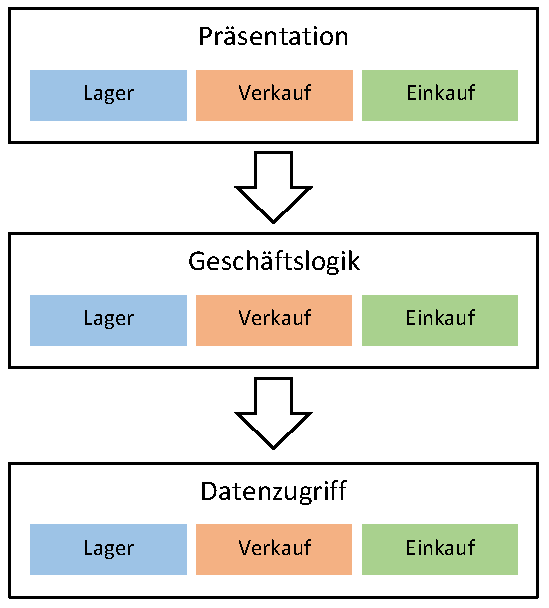
\includegraphics[width=0.8\linewidth]{layered-architecture}
	\caption{Drei-Schicht-Architektur}
	\label{fig:layered-architecture}
\endminipage
\minipage{0.5\textwidth}
  \centering
	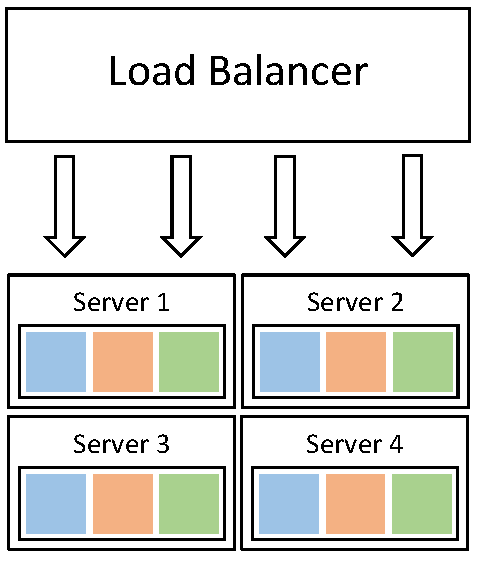
\includegraphics[width=0.76\linewidth]{monolith-scale}
	\caption{Skalieren einer monolithischen Anwendung}
	\label{fig:monolith-scale}
\endminipage
\end{figure}

\subsubsection{Nachteile und Schwierigkeiten}

Mit steigender Komplexität der Software kommen nach und nach Probleme zum Vorschein, die diesen Ansatz aufwändig oder sogar unpraktikabel machen. Eine der größten Herausforderungen bei der Entwicklung von Anwendungen mit globaler Reichweite ist die Skalierbarkeit. Die einzige Möglichkeit, eine monolithische Anwendung zu skalieren, ist auf mehreren Servern jeweils eine Instanz der Anwendung zu installieren und über einen Load-Balancer zu verbinden. Abbildung \ref{fig:monolith-scale} zeigt, wie ein solcher Aufbau aussehen kann. In vielen Einsatzgebieten ist dieser Ansatz aber nicht feingranular genug. Oft ist es sinnvoller, nur bestimmte Teile des Gesamtsystems zu skalieren.

Ein Monolith stößt aber nicht nur aus technischer Sicht auf Skalierbarkeitsprobleme, sondern auch aus organisatorischer Sicht. Alle Entwickler arbeiten zwangsläufig an der gleichen Codebasis, die dadurch enorme Größe annehmen kann. Kein einzelner Entwickler ist mehr in der Lage, die ganze Codebasis zu überblicken und zu beurteilen, welche Auswirkung eine Änderung haben kann. Das führt über kurz oder lang zur Verlangsamung der Entwicklungsgeschwindigkeit oder sogar zu völligem Stillstand.

Anforderungen an eine Software ändern sich häufig sehr rasch. Agile Softwareprozesse unterstützen dabei, die geänderten Anforderungen zeitnahe in die Software einfließen zu lassen. Für den Kunden \bzw Endbenutzer zählt nur die schnellstmögliche Umsetzung seiner neuen Anforderungen. In einer monolithischen Anwendung sind mehrere Geschäftsbereiche zusammengefasst. Somit muss die Anwendung immer als ganzes getestet und ausgerollt werden. Dadurch verlangsamt sich der gesamte Releasezyklus auf den langsamsten Teilbereich, obwohl vielleicht der geänderte Teilbereich schon längst fertiggestellt ist.

Hinter einer monolithischen Anwendung steht immer eine bestimmte Technologie oder eine Sammlung von mehreren Technologien, wie \zB Java EE oder ASP.NET. Somit müssen alle Teilbereiche der Anwendung auf die selben Technologien zurückgreifen. Für manche Teilbereiche könnte aber möglicherweise die Verwendung von alternativen Technologien und Speichersystemen große Vorteile bringen.

In diesem Abschnitt wurden einige der Hauptkritikpunkte am monolithischen Architekturmuster angeführt. Es mag den Anschein vermittelt haben, dass dieser Ansatz nicht mehr verwendet werden soll oder veraltet ist. Aber das ist so nicht der Fall. Viele Experten sind der Meinung, dass gerade am Anfang eines Projekts der monolithische Ansatz zu bevorzugen ist \cite{FowlerMolithFist}. Erst nachdem das Verständnis für die Domäne vorhanden ist und Anforderungen klarer sind, ist der fließende Übergang zu einer Microservice Architektur einfacher und sinnvoll. 

\section{Charakteristiken von Microservices}

Dieser Abschnitt beschreibt einige charakteristische Merkmale eines Microservice. Wie bereits erwähnt, gibt es keine eindeutige Definition eines Microservice. Daher ist es sinnvoller, allgemeine anerkannte Charakteristiken der Microservice-Architektur zu betrachten.
 
\citeauthor{FowlerMS} identifizierte in \cite{FowlerMS} neun Charakteristiken von Microservices. Obwohl diese Liste bereits sehr umfangreich ist, sind immer wieder sinnvolle Ergänzungen, wie in \cite{HorsdalMS} zu finden. Die nachfolgenden Abschnitte beschreiben eine repräsentative Auswahl dieser Charakteristiken.

\subsection{Organisation um Geschäftskompetenzen}

Normalerweise sind Softwareentwicklungsteams anhand ihrer technologischen Spezialisierung \zB in folgende Teams eingeteilt:

\begin{itemize}
	\item Front-End-Entwickler
	\item Backend-End-Entwickler
	\item Datenbank-Administratoren
	\item IT-Administratoren
\end{itemize}

Durch die Microservice-Kultur hat sich aber eine andere Art der Teamstrukturierung etabliert. Für jede Geschäftskompetenz ist genau ein Team, welches intern aus einer kleinen Anzahl an den eingangs genannten Technologieexperten besteht, verantwortlich. Damit soll die Identifizierung und das Verantwortungsbewusstsein jedes einzelnen Teammitglieds für den von ihm entwickelten und betriebenen Dienst gestärkt werden.

Was aber dennoch eine große Herausforderung bleibt, ist die Definition des Aufgabenbereichs eines einzelnen Teams. Die Identifikation und Abgrenzung der Geschäftskompetenzen eines Unternehmens ist eine sehr komplexe Aufgabe. Als Hilfsmittel lässt sich hier das \begin{english} Single-Responsibility-Principle\end{english} heranziehen \cite{MartinAgile}: 

\begin{english}
\begin{quote}
  \textit{A class should have only one reason to change.}
\end{quote}
\end{english}

Das aus der objektorientierten Programmierung bekannte Entwurfsprinzip kann auch im Kontext von Microservices angewandt werden. Es erweitert diesen Grundsatz von der Klassen-Ebene auf die Dienst-Ebene. Das heißt, jeder Dienst soll genau eine Fähigkeit realisieren. Damit ist sichergestellt, dass geänderte Geschäftsanforderungen so wenig wie möglich andere Microservices beeinflussen.

\subsection{Modularisierung durch Dienste}
\label{subsec:Componentization}

Seit Jahrzehnten strebt die Softwareentwicklungsbranche danach, komplexe Softwaresysteme einfach durch die Integration verschiedener Komponenten realisieren zu können. Durch die vielen über Jahre hinweg entwickelten Ansätze, ist leider auch der Begriff Komponente sehr überstrapaziert und hat dementsprechend viele unterschiedliche Bedeutungen. Beispielsweise kann in der objektorientierten Programmierung eine Klasse als Komponente betrachtet werden. Im Java-Umfeld werden \textit{Enterprise Java Beans} gerne als verteilte Komponenten bezeichnet. In anderen Bereichen wiederum wird der Begriff für ein Software-Modul verwendet.

Auch wenn die konkrete Umsetzung einer Komponente sehr vielfältig sein kann, haben alle Ansätze dieselben Ziele:

\begin{itemize}
	\item \textbf{Austauschbarkeit:} Es soll möglich sein, eine Komponente durch eine andere zu ersetzen. 
	\item \textbf{Wiederverwendbarkeit:} Eine entwickelte Komponente soll auch in anderen Systemen wiederverwendet werden können.
	\item \textbf{Aktualisierbarkeit:} Durch die Austauschbarkeit ist es automatisch möglich, eine Komponente durch eine neuere Version zu ersetzen, ohne den Rest der Anwendung zu beeinflussen.
\end{itemize}

Im Kontext der monolithischen Softwarearchitektur sind am häufigsten die Begriffe Modul oder Software-Bibliothek ein Synonym für den Begriff Komponente. Eine Anwendung besteht somit aus einer Menge von Modulen, die miteinander verbunden sind. Leider erfüllt dieser Ansatz die zuvor beschriebenen gewünschten Eigenschaften der Komponenten-Orientierung nicht ganz zufriedenstellend. Abhängigkeiten zwischen den einzelnen Modulen oder bestimmte Voraussetzungen an das Laufzeitsystem der monolithischen Anwendung können das Aktualisieren eines Moduls wesentlich erschweren. Somit sind die verwendeten Komponenten nicht völlig voneinander unabhängig, sondern haben versteckte Abhängigkeiten.

In einer Microservice-Architektur ist mit Komponente ein einzelner Dienst gemeint. Damit ist jede Komponente ein eigener Prozess, der über ein Kommunikationsprotokoll mit anderen Komponenten interagiert. Mit diesem Ansatz lassen sich die gewünschten Eigenschaften viel leichter realisieren.

\subsection{Dezentrale Datenverwaltung}

Eine monolithische Anwendung legt sehr häufig alle persistenten Daten in einer einzigen relationalen Datenbank ab. Jeder Programmteil greift einfach auf die benötigten Daten direkt zu. Dieser Ansatz ist in Abbildung \ref{fig:central-datastore} dargestellt. In einer Microservice-Architektur ist dieser Ansatz nicht mehr empfehlenswert. Persistente Daten eines bestimmten Geschäftsbereichs sollen nur von einem einzigen Dienst verwaltet werden. Direkter Zugriff auf diese Daten durch andere Dienste führt zu unerwünschten Abhängigkeiten. Andere Dienste müssen Daten über die öffentliche Schnittstelle des zuständigen Microservices abfragen oder verändern.

\begin{figure}[h]
  \centering
	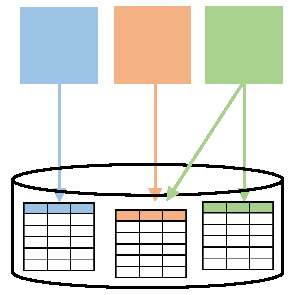
\includegraphics[width=0.3\textwidth]{central-datastore}
	\caption{Zentraler Datenspeicher}
	\label{fig:central-datastore}
\end{figure}

Wenn jeder Dienst wie in Abbildung \ref{fig:polyglot-persistnace} seinen eigenen Datenspeicher besitzt, kann für die Erfüllung seiner Aufgabe der optimale Speichermechanismus ausgewählt werden. Beispielsweise können Daten mit komplexen Beziehungen in einer Graphdatenbank abgelegt werden, einfache Daten jedoch in einem schnellen Key-Value-Speicher.

\begin{figure}[h]
  \centering
	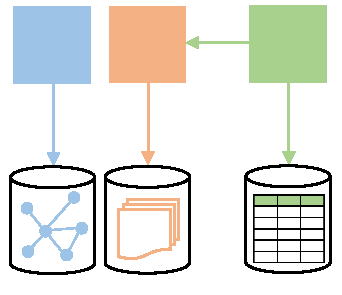
\includegraphics[width=0.3\textwidth]{polyglot-persistance}
	\caption{Polyglot Persistance}
	\label{fig:polyglot-persistnace}
\end{figure}

Auch eine monolithische Anwendung könnte Gebrauch von mehreren Datenbanken machen. Dieser Ansatz ist unter dem Namen Polyglot Persistence bekannt \cite{FowlerPP}. Aus teilweise sehr vielfältigen Gründen ist er aber selten anzutreffen. Dazu zählen beispielsweise folgende:

\begin{itemize}
  \item Die IT-Strategie einiger Unternehmen sehen nur die Verwendung ganz bestimmter Datenbanken vor.
	\item Bereits getätigte Investitionen in bestehende Datenbanksysteme müssen amortisiert werden.
	\item Angst vor dem Betrieb einer Datenbank, für die noch nicht die notwendige Erfahrung aufgebaut wurde.
\end{itemize}

Für Systeme mit hohen Anforderungen an die Verfügbarkeit ist die Verwendung einer einzigen Datenbank nicht ausreichend. Denn eine einzige Datenbank stellt einen kritischen \textit{Single Point of Failure} dar.

\subsection{Automatisierung}

Für ein erfolgreiches System, das aus Microservices besteht, ist ein hoher Grad an Automatisierung erforderlich. Durch die große Anzahl an Komponenten im System, muss die Anzahl an manuell erforderlichen Schritten sehr gering sein. Ansonsten ist der Aufwand für das Aktualisieren, Ausrollen, Testen und Überwachen viel zu groß.

Um von den Vorteilen der Microservice-Architektur gegenüber einer monolithischen profitieren zu können, ist es unabdingbar, dass jeder Dienst einzeln ausgerollt werden kann. Denn nur damit sind die Entwicklungs- und Releasezyklen der einzelnen Dienste im Gesamtsystem voneinander unabhängig.

Wenn jeder Dienst einzeln ausgerollt werden kann, ist es auch möglich, unterschiedliche Versionen gleichzeitig zu betreiben. Somit kann eine neue Version getestet werden und erst wenn diese Testphase erfolgreich abgeschlossen ist, der gesamte Datenverkehr auf diesen Dienst umgeleitet werden. Bei Problemen kann schnell der ursprüngliche Zustand wiederhergestellt werden. Insgesamt mindert ein derartiges Vorgehen das Risiko eines großen Big-Bang-Deployments.

Damit dieser Ansatz funktioniert, müssen die Dienste einige Anforderungen erfüllen. Jeder Dienst steht mit einigen anderen in Verbindung. Wenn nun eine neue Version eines Dienstes ausgerollt wird, muss dessen Schnittstelle abwärtskompatibel sein, da seine Konsumenten noch die alte Schnittstelle verwenden. Fehlertoleranz ist eine weitere wichtige Eigenschaft, da während eine neue Version ausgerollt wird, der Dienst kurzzeitig nicht verfügbar sein kann.

\subsection{Größe}

Wie der Name bereits suggeriert, soll ein Microservice klein sein. Das sollte schon durch die Anwendung des \textit{Single-Responsibility} Prinzips aus Abschnitt \ref{subsec:Componentization} gegeben sein. Wie groß ein Dienst genau sein soll, lässt sich aber aus vielen Gründen schwer festlegen. Die Anzahl der Quelltextzeilen ist ein schlechtes Maß für die Größe, da sie je nach Programmiersprache stark variiert. Schon aussagekräftiger ist die benötigte Zeitdauer für die Entwicklung des Dienstes. Aber auch diese Kennzahl kann trügerisch sein. Beispielsweise kann man mit der Verwendung von externen Bibliotheken eine große Zeitersparnis erzielen. Jedoch inkludiert der Service dann auch die Komplexität dieser Bibliothek.

Eine genaue domänen-unabhängige Größenangabe ist praktisch nicht möglich. Es kann lediglich ein grober Rahmen abgesteckt werden. Ein Microservice sollte eine Entwicklungszeit von mehreren Wochen nicht übersteigen.

Neben quantitativen Kennzahlen sind oft subjektive Kriterien erforderlich. Eine davon ist, dass ein einzelner Entwickler die gesamte Funktionalität eines Dienstes noch im Kopf behalten können muss. Sobald es keinen einzelnen Menschen mehr gibt, der alle Aspekte des Dienstes auf einmal überschauen kann, ist er auf jeden Fall zu groß. Meistens aber haben erfahrene Architekten und Entwickler ein sehr gutes Gefühl, ab welcher Größe ein Dienst zu groß ist.

\section{Vorteile}

Ein neuer Softwareentwicklungsansatz setzt sich nur dann durch, wenn er auch einen erkennbaren Mehrwert bietet. Dieser Abschnitt zeigt einige der Vorteile, die durch den intelligenten Einsatz einer Microservice-Architektur entstehen können \cite{fowlerMSTradeOffs,newman2015building}.

Es ist wichtig zu verstehen, dass die Vorteile, die durch Microservices entstehen, erst ab einer gewissen Größe \bzw Komplexität des Gesamtsystems zum Tragen kommen. In einfachen Softwaresystemen steht die Komplexität der Microservice-Architektur in keinem angemessenen Verhältnis zu deren Vorteilen \cite{fowlerMSPremium}.

\subsection{Heterogener Technologieeinsatz}

Beim monolithischen Ansatz sind die Technologieentscheidungen äußerst eingeschränkt \cite{fowlerMSTradeOffs}. Nachdem die Haupttechnologie festlegt ist, kann aus diesem Korsett nur noch geringfügig ausgebrochen werden. Aber nicht für alle Aufgaben muss der eingeschlagene Weg auch der optimale sein.

Hier kommt ein wesentlicher Vorteil von Microservices zum Tragen. Da jeder Dienst eine kleine autonome Komponente ist, sind für jeden Dienst unterschiedliche sinnvolle Technologieentscheidungen möglich. Selbst die Wahl des Speichermechanismus kann individuell erfolgen. Die eingesetzte Technologie kann beispielsweise von der Aufgabenstellung oder den Fähigkeiten der Teammitglieder abhängig gemacht werden. Damit werden die Technologieentscheidungen nicht mehr von zentraler Stelle gesteuert, sondern die Kompetenz in die einzelnen Teams verlagert.

Die Macht der freien Technologieauswahl ist aber mit Bedacht einzusetzen. Es kann für ein System auch kontraproduktiv sein, wenn zu viele Technologien eingesetzt werden, die womöglich noch nicht einmal ein stabiles Stadion erreicht haben. Daher macht die Definition von Team-übergreifenden Richtlinien zur Technologieauswahl durchaus Sinn. Der entscheidende Vorteil gegenüber dem monolithischen Ansatz ist aber die Wahlfreiheit, auch nach dem Start der Entwicklung.

\subsection{Robustheit}

Durch den hohen Modularisierungsgrad in einer Microservice-Architektur herrscht ein ganz anderes Verständnis bezüglich der Verfügbarkeit von einzelnen Komponenten, wie in einer monolithischen Architektur. In einer monolithischen Anwendung befinden sind nämlich alle Komponenten in einem einzelnen Prozess. Daher kann ein Entwickler davon ausgehen, dass alle Komponenten immer verfügbar sind. Nicht so in einer Microservice-Architektur. Hier muss jederzeit davon ausgegangen werden, dass Dienste nur eingeschränkt oder gar nicht verfügbar sind.

Wenn eine monolithische Anwendung ausfällt, ist das ganze System nicht mehr verwendbar. Im Gegensatz dazu kann das Gesamtsystem trotz des Ausfalls eines oder mehrere Microservices, zumindest eingeschränkt, weiterlaufen.

\subsection{Einfaches Deployment}

Jedes Release einer großen monolithischen Anwendung stellt ein gewisses Risiko dar. Daher passieren solche Releases in eher großen Abständen. In einem agilen Umfeld sind derartige lange Releasezyklen nicht tragbar. Außerdem kann jede kleine Fehlfunktion das ganze Deployment zum Scheitern bringen.

Mit Microservices ist es möglich, jeden Dienst einzeln auszurollen. Damit ist die Auswirkung aus Sicht des Gesamtsystems viel geringer. Wenn der Dienst nach dem Ausrollen einen Fehler aufweist, kann nur dieser eine Dienst auf den Ausgangszustand zurückgesetzt werden.

Auch die Abhängigkeiten zwischen den einzelnen Teams ist durch den Microservice-Ansatz reduziert. Ein Team kann ihren Service um Funktionalität erweitern und sofort ausrollen. Andere Teams, die diese Funktionalität verwenden wollen, können erst dann neu ausrollen wenn ihr Dienst stabil ist. Dafür ist es aber notwendig, dass alle Dienste ihre Schnittstellen stets rückwärtskompatibel halten.

Die in diesem Abschnitt beschriebenen Vorteile einer Microservices Architektur sind keinesfalls allumfassend. Je nach Einsatzgebiet kommen möglicherweise auch andere Vorteile stärker zum Tragen als die hier angeführten. Um von den Vorteilen profitieren zu können, ist eine ordentliche Umsetzung dieses Architekturmusters aber unumgänglich. Denn ansonsten hat man zwar die gesamte Komplexität die Microservices mit sich bringen, jedoch nicht die gewünschten Vorteile.

\section{SOA}

Ein kontrovers diskutiertes Thema im Bezug auf Microservices ist die Beziehung zu Service-orientierter Architektur, kurz SOA. Das abstrakte Architekturmuster SOA wurde bereits 1996 in \cite{schulte1996service} beschrieben und hat sich seither ständig weiterentwickelt.

Auch bei SOA ist es schwer, eine genaue Definition zu geben. Grundsätzlich handelt es sich dabei um eine lose gekoppelte Softwarearchitektur, in der die Komponenten der Software in Form von autonomen Diensten, um die Geschäftsprozesse gestaltet werden \cite{soaRW}. Neben dieser einfachen informellen Definition hafteten sich über die Jahre immer neue Konzepte an den Begriff an. Mittlerweile verbinden viele Architekten konkrete Technologien mit dem eigentlich abstrakten Konzept. Sehr häufig zählen dazu Technologien, wie SOAP, WSDL, WS-* Protokolle oder auch Nachrichten-orientierte Middleware Lösungen, wie ESB \cite{fowlerGoTo}. Aus diesem Grund stößt dieses Muster oft auf Ablehnung, da fälschlicherweise viele komplexe Technologien damit in Verbindung gebracht werden.

\citeauthor{newman2015building} beschreibt in \cite{newman2015building}, dass Microservices und SOA so wie Scrum und agile Softwareentwicklung miteinander in Beziehung stehen. Scrum ist eine konkrete Form von agiler Softwareentwicklung. So sind auch Microservices ein bestimmter Stil SOA umzusetzen. Da alle Konzepte einer Microservice Architektur auch in SOA enthalten sind, können Microservices als Teilmenge und Konkretisierung von SOA verstanden werden.

Oft wird SOA dafür kritisiert, viel zu abstrakt und breit gefächert zu sein. Es gibt viel zu wenig konkrete Hilfestellungen, beispielsweise für den Entwurf von Service-Grenzen oder die Bestimmung der Service-Größe. Das Konzept der Microservices hingegen wurde für einen bereits existierenden Stil der Anwendungsentwicklung nachträglich geprägt. Bei SOA hingegen wurde zuerst das Konzept definiert.

\section{Zusammenfassung}

In diesem Abschnitt wurden Microservices als um Geschäftskompetenzen entworfene, lose gekoppelte und autonome Dienste in einer service-orientierten Architektur, definiert. Der Begriff Microservices dient als Sammelbegriff für viele Konzepte, die sich um dieses Architekturmuster scharen. Im Gegensatz zu SOA ist die Vorstellung, was Microservices sind, viel konkreter, obwohl auch Microservices immer noch viel Interpretationsspielraum offenlassen.

Monolithischen Anwendung bündeln sämtliche Funktionalität eines Systems in einem einzigen großen ausführbaren Prozess. Bei der Microservice-Architektur stehen wichtige Funktionalitäten als eigenständiger Dienst zur Verfügung. Das ermöglicht großen Teams die Arbeit an komplexen Aufgaben, ohne sich gegenseitig zu stören. Damit ist es jedem Team selbst überlassen, die optimalen Technologieentscheidungen zu treffen, den Releasezyklus des Dienstes zu bestimmen und den Dienst in robuster Art und Weise zu implementieren.

Den Vorteilen der Microservice-Architektur steht aber eine nicht zu unterschätzende Komplexität gegenüber. Beispielsweise die Orchestrierung aller einzelnen Dienste zu einer Einheit stellt eine große Herausforderung dar. Außerdem fließt viel Arbeit in die saubere Definition der Schnittstellen zwischen den Diensten ein. Einfache Anpassungen können schnell ausarten, da sie mehrere Dienste betreffen können. 

Nichtsdestotrotz hat das Microservice-Architekturmuster in vielen Einsatzgebieten seine Vorzüge. Am Beginn einer Microservice-Architektur sollte eine ausführliche Aneignung des erforderlichen Domänenwissens stehen. Oft funktioniert das nur durch den Start der Entwicklung mit einer monolithischen Architektur. Das Ziel sollte eine evolutionäre Architektur sein. Eine monolithische Architektur kann mit steigenden Verständnis für die Servicegrenzen leicht in eine Microservice-Architektur überführt werden.